\documentclass[journal]{IEEEtran}
\usepackage[a5paper, margin=10mm, onecolumn]{geometry}
\usepackage{tfrupee}
\usepackage{amsmath, amssymb, amsfonts, amsthm}
\usepackage{algorithmic}
\usepackage{graphicx}
\usepackage{textcomp}
\usepackage{xcolor}
\usepackage{txfonts}
\usepackage{listings}
\usepackage{enumitem}
\usepackage{mathtools}
\usepackage{gensymb}
\usepackage{comment}
\usepackage[breaklinks=true]{hyperref}
\usepackage{tkz-euclide} 
\usepackage{listings}
\usepackage[latin1]{inputenc}                                
\usepackage{color}                                            
\usepackage{array}                                            
\usepackage{longtable}                                       
\usepackage{calc}                                             
\usepackage{multirow}                                         
\usepackage{hhline}                                           
\usepackage{ifthen}                                           
\usepackage{lscape}
\newcommand{\myvec}[1]{\begin{pmatrix} #1 \end{pmatrix}}

\begin{document}

\bibliographystyle{IEEEtran}
\vspace{3cm}

\title{NCERT-8.1.ex3}
\author{EE24BTECH11042 - SRUJANA}
{\let\newpage\relax\maketitle}

\renewcommand{\thefigure}{\theenumi}
\renewcommand{\thetable}{\theenumi}
\setlength{\intextsep}{10pt} 

\numberwithin{equation}{enumi}
\numberwithin{figure}{enumi}
\renewcommand{\thetable}{\theenumi}

\textbf{QUESTION}:\\

Find the area of the region bounded by the curve $y = x^2$ and the line y=4

\textbf{Theoretical Solution}:\\

Intersection points are 
\begin{align}
  4 = x^2 \implies x = \pm 2
\end{align}

Area 
\begin{align}
    \int_{-2}^{2} f(x) \, dx\\
    f(x) = 4 - x^2\\
    \int_{-2}^{2} (4-x^2) \, dx\\
    \left[ 4x - \frac{x^3}{3} \right]_{-2}^2 = \left( 8 - \frac{8}{3} \right) - \left( -8 + \frac{8}{3} \right)\\
    \text{Area} =  \frac{32}{3} = 10.666
\end{align}

\textbf{Trapezoidal method}

The trapezoidal rule approximates the integral using the formula:\\
\begin{align}
    A \approx \frac{h}{2} \left[ f(x_0) + 2 \sum_{i=1}^{n-1} f(x_i) + f(x_n) \right]
\end{align}
where:\\
\begin{enumerate}
   \item $h=\frac{b-a}{n}$ is the width of each subinterval.
   \item $f(x) = 4-x^2$.
   \item $a=-2,b=2$.
   \item $n$ is the number of subintervals.
\end{enumerate}
Taking trapezoid shaped strips of small area and adding them all up.. Say we have to
find the area of $y(x)$ from $x=x_0$ to $x = x_n$,discretize points on the x axis $x_0,x_1,x_2,...,x_n$ such that they are equally spaced with step-size h.Sum of all trapezoidal areas is given by,
\begin{align}
    A &= \frac{1}{2}h\left[y(x_1)+y(x_0)\right]+\frac{1}{2}h\left[y(x_2)+y(x_1)\right]+\frac{1}{2}h\left[y(x_3)+y(x_2)\right]+\dots+\frac{1}{2}h\left[y(x_n)+y(x_{n-1})\right] \\
    &= h\left[\frac{1}{2}\left(y(x_0)+y(x_n)\right)+y(x_1)+y(x_2)+\dots+y(x_{n-1})\right]
\end{align}

Let $A(x_n)$ be the area enclosed by the curve $y(x)$ from $x=x_0$ to $x=x_n$:
\begin{align}
    A(x_{n}+h) &= A(x_n) + \frac{1}{2}h\left[y(x_{n}+h)+y(x_n)\right]
\end{align}

We can repeat this till we get the required area:
\begin{align}
    A_{n+1} &= A_n + \frac{1}{2}h\left[y_{n+1}+y_n\right]
\end{align}

We can write $y_{n+1}$ in terms of $y_n$ as:
\begin{align}
    y_{n+1} &= y_n + h\cdot y^{\prime}_n
\end{align}

Substituting this into the equation, we get:
\begin{align}
    A_{n+1} &= A_n +\frac{1}{2}h\left[\left(y_n+h\cdot y^{\prime}_n\right)+y_n\right] \\
    A_{n+1} &= A_n + hy_n + \frac{1}{2}h^2y^{\prime}_n \\
    A_{n+1} &= A_n + h(4 - x_n^2) + \frac{1}{2}h^2(-2x_n) \\
    x_{n+1} &= x_n + h
\end{align}
By assuming some value for n area is obtained

\begin{figure}[h!]
   \centering
   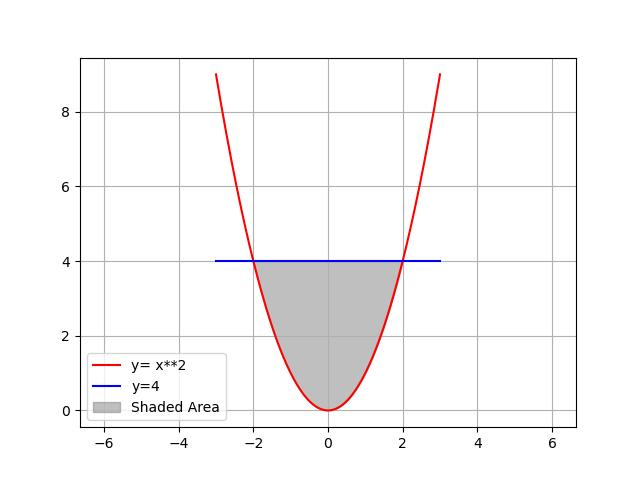
\includegraphics[width=\columnwidth]{fig/fig.jpg}
\end{figure}



\end{document}

